% ablation.tex — \input'd from thesis appendix
%
% Status: A-axis complete. Four variants: A0 (unpruned), A1 (vertex adjacency),
%   A2 (directed ω₀), A3 (Reeb-flow feasibility).
%
% Sources: experiments/ablation/ablation.jsonl (generated by ablation.rs),
%   experiments/ablation/ablation_timing.png (generated by ablation.py).
%
% Mathematical references used here (all Jörn-approved in commit 0839595):
%   lem:adjacency-constraint — consecutive facets with positive dwell time are adjacent
%   cor:adjacency-pruning — discard (S,σ) with non-adjacent consecutive pairs

\subsection{Adjacency Graph Pruning}
\label{sec:ablation-pruning}

We iteratively refine the adjacency graph used to prune the search space
of the HK2017 algorithm, starting from the unpruned baseline and adding
strictly stronger conditions at each step. Each variant is tested on a
fixed dataset of 38 polytopes to verify correctness and measure speedup.

\paragraph{Variants.}
Table~\ref{tab:ablation-variants} lists the four adjacency-graph variants.
Each adds a necessary condition for the existence of a valid orbit transition
$F_i \to F_j$, building on all previous conditions.

\begin{table}[h]
\centering
\begin{tabular}{lp{9cm}}
\toprule
Variant & Pruning condition for transition $F_i \to F_j$ \\
\midrule
A0 & None (unpruned): exhaustive search over all $(S, \sigma)$ \\
A1 & Vertex adjacency: $F_i \cap F_j \neq \varnothing$, checked via shared polytope vertices (Corollary~\ref{cor:adjacency-pruning}) \\
A2 & Directed $\omega_0$: A1 and $\omega_0(n_i, n_j) \ge 0$, ensuring the Reeb flow on $F_i$ carries the orbit toward~$F_j$ \\
A3 & Reeb-flow feasibility: A2 and $\exists\, x \in F_i \cap F_j$ with $x - \varepsilon R_i \in F_i$ and $x + \varepsilon R_j \in F_j$, ensuring other halfspaces do not block the transition \\
\bottomrule
\end{tabular}
\caption{Adjacency graph variants, each strictly stronger than the previous.
  The pruning condition applies to each consecutive pair in a candidate ordering
  $\sigma$; orderings that violate any edge condition are discarded.}
\label{tab:ablation-variants}
\end{table}

\paragraph{Directed symplectic condition (A2).}
For a physical orbit transition $F_i \to F_j$ at a ridge point $x \in F_i \cap F_j$,
the backward Reeb flow $x - \varepsilon R_i$ must remain in~$K$.
Checking the half-space constraint for facet~$j$ gives
$\omega_0(n_i, n_j) \ge 0$ as a necessary condition;
the forward flow $x + \varepsilon R_j$ on~$F_j$ gives the same condition
by antisymmetry of~$\omega_0$.
% [TODO: JÖRN - verify this derivation. Agent derived and confirmed empirically
%  on all 38 test polytopes. But the derivation needs mathematical verification.]

\paragraph{Reeb-flow feasibility (A3).}
A3 strengthens A2 by also checking the half-space constraints of all \emph{other}
facets $F_k$ ($k \neq i, j$).
For each $k$, we define a ``blocking set''
$B = \{k \notin \{i,j\} : \omega_0(n_i, n_k) < 0 \text{ or } \omega_0(n_j, n_k) > 0\}$,
and check whether $F_i \cap F_j$ contains a point satisfying
$n_k \cdot x < h_k$ for all $k \in B$.
This is a linear feasibility problem on the 2-dimensional ridge,
solved via Fourier--Motzkin elimination.
The $O(F^4)$ precomputation cost is negligible compared to the exponential search.

\paragraph{Ridge sufficiency.}
The following lemma shows that A2 is already sufficient when
the two facets share a ridge (2-dimensional face).
In particular, A3 can only prune beyond A2 at non-simple vertices.

\begin{lemma}[Ridge sufficiency for orbit transitions]
\label{lem:ridge-sufficiency}
Let $K \subset \mathbb{R}^4$ be a convex polytope with facets
$F_1, \ldots, F_N$, outward unit normals~$n_k$, and support values~$h_k$.
Write $R_k = J_0 n_k$ for the characteristic direction on~$F_k$.
If\/ $F_i \cap F_j$ is a 2-dimensional face (ridge) of~$K$ and
$\omega_0(n_i, n_j) \ge 0$, then there exist $x \in F_i \cap F_j$
and $\varepsilon > 0$ such that
\[
  x + t\, R_i \in K \;\;\text{for all } t \in [-\varepsilon, 0],
  \qquad
  x + t\, R_j \in K \;\;\text{for all } t \in [0, \varepsilon].
\]
\end{lemma}

\begin{proof}
Since $F_i \cap F_j$ is a ridge, its relative interior is nonempty.
Pick any $x_0 \in \operatorname{relint}(F_i \cap F_j)$.
Then $n_i \cdot x_0 = h_i$, $n_j \cdot x_0 = h_j$, and
$n_k \cdot x_0 < h_k$ for all $k \notin \{i, j\}$.
Set $\delta = \min_{k \notin \{i,j\}} (h_k - n_k \cdot x_0) > 0$.

We check $n_k \cdot \gamma(t) \le h_k$ for all~$k$ on
both trajectory segments, using
$n_k \cdot R_\ell = \langle J_0 n_\ell, n_k \rangle = \omega_0(n_\ell, n_k)$.

\emph{Approach} ($\gamma(t) = x_0 + t\, R_i$, $t \in [-\varepsilon, 0]$):
\begin{itemize}
  \item $k = i$: \;
    $n_i \cdot \gamma(t)
      = h_i + t \,\omega_0(n_i, n_i) = h_i$,
    since $\omega_0$ is antisymmetric.
  \item $k = j$: \;
    $n_j \cdot \gamma(t)
      = h_j + t \,\omega_0(n_i, n_j) \le h_j$,
    since $t \le 0$ and $\omega_0(n_i, n_j) \ge 0$.
  \item $k \notin \{i,j\}$: \;
    $n_k \cdot \gamma(t) \le (h_k - \delta) + \varepsilon \,|\omega_0(n_i, n_k)| < h_k$
    for small~$\varepsilon$.
\end{itemize}

\emph{Departure} ($\gamma(t) = x_0 + t\, R_j$, $t \in [0, \varepsilon]$):
\begin{itemize}
  \item $k = j$: \; $n_j \cdot \gamma(t) = h_j$ (same argument).
  \item $k = i$: \;
    $n_i \cdot \gamma(t)
      = h_i + t \,\omega_0(n_j, n_i)
      = h_i - t \,\omega_0(n_i, n_j) \le h_i$,
    since $t \ge 0$ and $\omega_0(n_i, n_j) \ge 0$.
  \item $k \notin \{i,j\}$: \; same bound with $\omega_0(n_j, n_k)$ in place of $\omega_0(n_i, n_k)$.
\end{itemize}
Setting $\varepsilon = \delta\, / \bigl(1 + \max_k\, |\omega_0(n_i, n_k)|
+ \max_k\, |\omega_0(n_j, n_k)|\bigr)$ completes the proof.
\end{proof}

\begin{corollary}[A2 = A3 for simple polytopes]
\label{cor:a2-equals-a3-simple}
If every pair of adjacent facets of~$K$ shares a ridge,
then the~A2 and~A3 pruning conditions are equivalent.
In particular, this holds for all simple polytopes
and for all Lagrangian products $P \times Q$ of convex polygons.
\end{corollary}

\begin{proof}
If $F_i \cap F_j$ is always a ridge whenever it is nonempty,
Lemma~\ref{lem:ridge-sufficiency} shows that the A2 condition
$\omega_0(n_i, n_j) \ge 0$ already implies A3 feasibility.
For simple 4-polytopes, each vertex lies on exactly four facets,
so any two facets that share a vertex share a $4 - 2 = 2$ dimensional
face.
For Lagrangian products $P \times Q$ of convex polygons,
each pair of facets that intersects shares a 2-face:
two facets from the same factor share a ``vertex $\times$ polygon''
face, and two facets from different factors share an
``edge $\times$ edge'' face.
\end{proof}

\begin{example}[Non-simple polytope where A3 prunes beyond A2]
\label{ex:a3-prunes}
Consider the ``shaved hypercube''
\[
  K = \{\, x \in \mathbb{R}^4 : -2 \le x_i \le 0 \;\forall\, i,
  \quad x_2 \le x_1 \,\}.
\]
This polytope has $9$ facets and $12$ vertices, of which $8$
are non-simple (lying on $5$ facets).
The facets $F_1\colon (x_2 \le 0)$ and $F_2\colon (x_3 \le 0)$
share only a 1-dimensional edge:
the shaving constraint $x_2 \le x_1$ combined with $x_1 \le 0$
forces $x_1 = x_2 = 0$ on $F_1 \cap F_2$.
Since $\omega_0(n_1, n_2) = 0 \ge 0$, the A2 condition allows
the transition $F_1 \to F_2$.
However, the shaving facet $F_4$ (with normal $(-1, 1, 0, 0)/\sqrt{2}$)
is tight on the entire edge and belongs to the A3 blocking set
(since $\omega_0(n_2, n_4) = 1/\sqrt{2} > 0$),
so the A3 feasibility check fails.
In total, A3 prunes 8 directed edges that A2 allows.
\end{example}

\paragraph{Test polytopes.}
Table~\ref{tab:ablation-dataset} describes the 38 test polytopes.
Random polytopes use a fixed seed (42) and height range $h \in [0.5, 2.0]$.

\begin{table}[h]
\centering
\begin{tabular}{llrp{5.5cm}}
\toprule
Group & $F$ & Count & Description \\
\midrule
Random generic    & 5--8 & 20 & 5 random 4-polytopes per facet count \\
Random Lagrangian & 6--8 & 15 & 5 random products per pair:
  $\triangle{\times}\triangle$,
  $\triangle{\times}\square$,
  $\square{\times}\square$ \\
Regression cases  & 7--8 &  3 & Fixed polytopes triggering degenerate KKT systems \\
\bottomrule
\end{tabular}
\caption{Test polytope dataset. All random polytopes use seed~42, $h \in [0.5, 2.0]$.
  Regression cases: $\triangle{\times}\square$ at $\theta{=}0^\circ$ and
  $\square{\times}\square$ at $\theta{=}0^\circ$ trigger rank-deficient KKT systems;
  the hypercube exercises the LU fast path.}
\label{tab:ablation-dataset}
\end{table}

\paragraph{Correctness.}
All four variants return identical capacities on all 38 test polytopes (maximum
absolute difference $< 10^{-8}$).
This confirms that no pruning variant discards the optimal orbit on this dataset.

The three regression cases additionally verify correct handling of degenerate
KKT systems:
$\triangle{\times}\square$ at $\theta{=}0^\circ$ (expected $3\sqrt{2}/2 \approx 2.121$) and
$\square{\times}\square$ at $\theta{=}0^\circ$ (expected $2.0$) both require a null-space search
when the LU factorization detects rank deficiency;
the hypercube (expected $4.0$) is solved by the LU fast path without SVD.
All three capacities match their expected values to within $10^{-6}$.

\paragraph{Speedup.}
Table~\ref{tab:ablation-speedup} shows mean computation times.
The main speedup comes from the directed $\omega_0$ condition~(A2), which prunes
${\sim}99\%$ of candidate orderings at $F = 8$:
${\sim}130\times$ over A0 for generic polytopes, and
${\sim}36\times$ for Lagrangian products (whose structured normals have more
$\omega_0 = 0$ pairs, limiting directed pruning effectiveness).
A3 provides no additional pruning beyond A2 on this dataset; this is expected
for polytopes with $F \le 8$, where ridges are in sufficiently general position
that the $\omega_0$ condition alone captures all blocking.
Standard deviations are shown in Figure~\ref{fig:ablation-timing}.

\begin{table}[h]
\centering
\begin{tabular}{llrrrr}
\toprule
Group & $F$ & A0 (ms) & A1 (ms) & A2 (ms) & A3 (ms) \\
\midrule
Generic    & 5 &   0.5 &   0.5 &  0.1 &  0.1 \\
           & 6 &   3.2 &   2.5 &  0.2 &  0.2 \\
           & 7 &  26.9 &  13.7 &  0.6 &  0.6 \\
           & 8 & 234.5 &  74.0 &  1.8 &  1.7 \\
\midrule
Lagrangian & 6 &   3.0 &   2.9 &  0.7 &  0.7 \\
           & 7 &  27.3 &  14.6 &  2.1 &  2.1 \\
           & 8 & 239.4 &  79.4 &  6.8 &  6.6 \\
\bottomrule
\end{tabular}
\caption{Mean computation time (ms) by adjacency variant,
  $n = 5$ samples per group per facet count.
  The directed $\omega_0$ condition (A2) provides the dominant speedup:
  ${\sim}130\times$ over A0 at $F = 8$ (generic).
  A3 adds no further pruning on this dataset.}
\label{tab:ablation-speedup}
\end{table}

\begin{figure}[h]
\centering
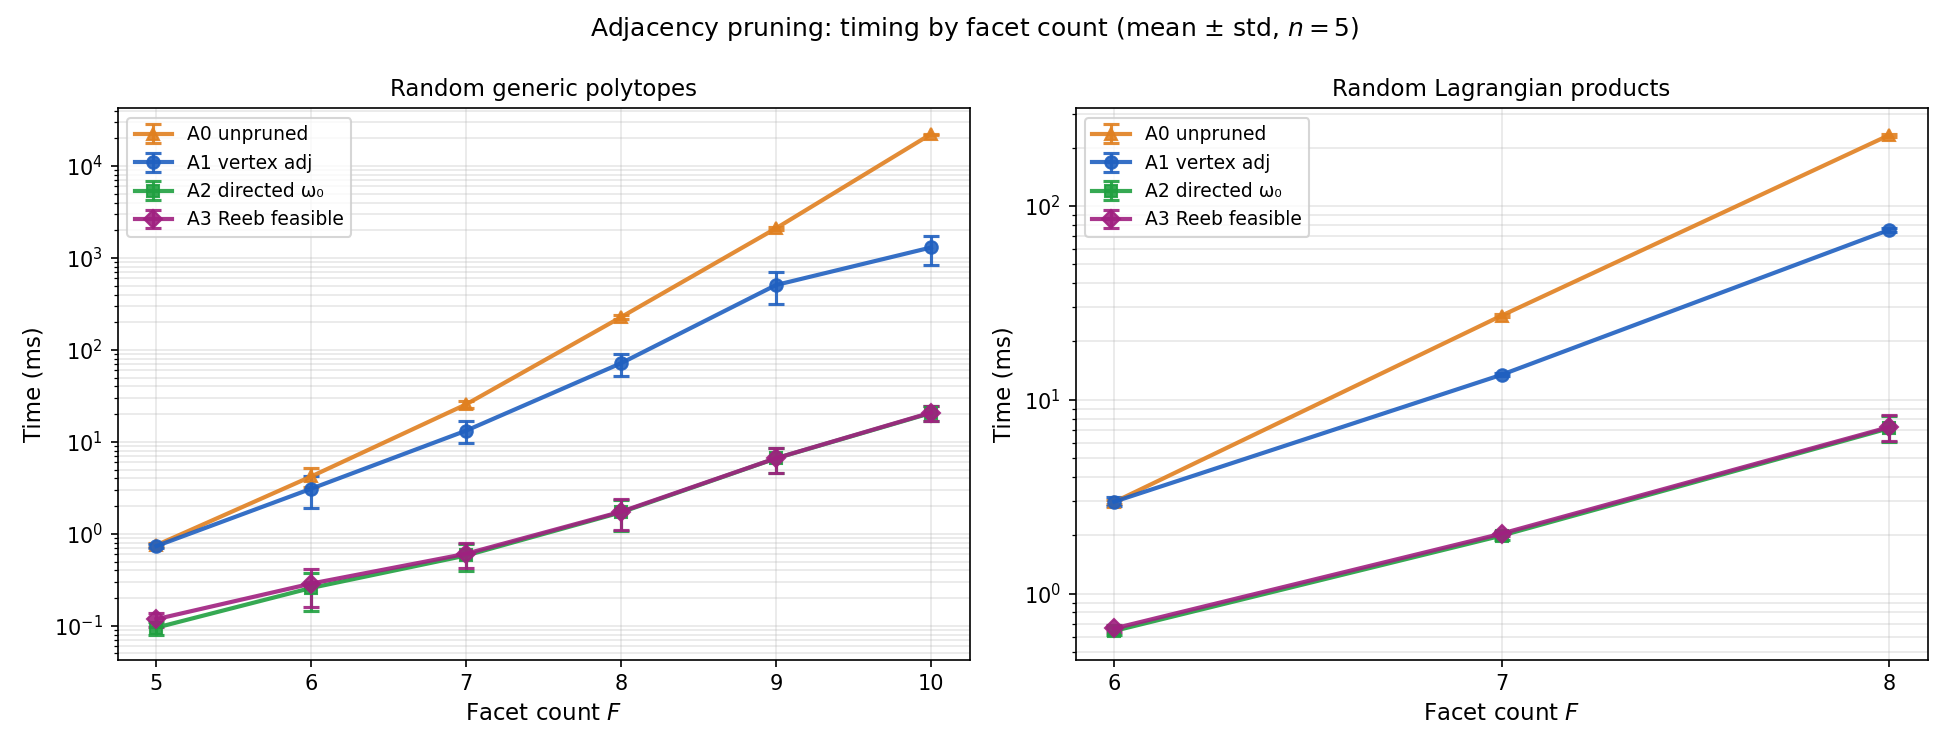
\includegraphics[width=0.95\textwidth]{../experiments/ablation/ablation_timing.png}
\caption{Adjacency pruning: timing by facet count,
  mean $\pm$ std ($n=5$).
  Left: random generic polytopes. Right: random Lagrangian products.
  A2~and~A3 (green squares and purple diamonds) overlap almost exactly,
  confirming that the $\omega_0$ condition captures all prunable transitions
  on this dataset.}
\label{fig:ablation-timing}
\end{figure}
